\section{Brief overview and description of analysis codes}

\subsection{VDFs}
The analysis is done with three separate programs which I have written in the Python programming language. Amongst other things they agree with cosmological simulations about virial radius which tend to be $r_{vir}=10r_{-2}$, with $r_{-2} = \frac{r_s}{2}$ (for a Hernquist profile). For a NFW profile, $r_s=r_{-2}$. To see the programs, look under appendices D, E and F, where there is also a short introduction to each program. Comment lines are included into the code, to clarify each step taken. In this section I will simply attempt to highlight the most prominent features of each of these codes. For the first code, 'Read.py', the central part is the following for-loop which we shall now investigate further: \\ 

\begin{pythonstyle}
\begin{lstlisting}[language=Python]
# Divide the structure into logarithmic radial bins
for i in range(0, int(nr_binning_bins)):      # loop over the number of bins 
    min_R_bin_i = binning_arr_lin_log10[i]    # start of bin 
    max_R_bin_i = binning_arr_lin_log10[i+1]  # end of bin 
    posR_par_inside_bin_i = np.where((R>min_R_bin_i) & (R<max_R_bin_i))[0] # position of particles inside a radial bin 
    # number of particles inside a radial bin:    
    nr_par_inside_bin_i   = len(posR_par_inside_bin_i)                     
    # Volume of cluster: 
    Volume_cl = (4./3.)*np.pi*(max_R_bin_i**3 - min_R_bin_i**3) 
    den_cl = nr_par_inside_bin_i/Volume_cl # number density 
    rho_cl = m*den_cl                      # density (m is the mass of each particle, m = M/N = 1/N)
    # save to lists 
    density_arr.append(den_cl) 
    Volume_arr.append(Volume_cl) 
Invers_Volume_arr = np.log10(np.divide(np.ones(len(Volume_arr)),Volume_arr)) 
\end{lstlisting}
\end{pythonstyle}

After cutting the cluster structure up into logarithmic linear radial bins, each bin contains a certain number of particles whose various physical quantities is then averaged,e.g. the number density given by number of particles in each bin divided by the volume of this spherical shell. The number of particles for a certain bin, i,  is found by taking the length of the array containing all particles inside  bin\_i. The volume of a spherical shell in general is just the volume of the remainder of the whole sphere´s volume after subtracting the volume of the inside sphere (with radius equal to the start value of the bin radius). This is then used in the line above which writes  \\
\begin{pythonstyle}
\begin{lstlisting}[language=Python]
Volume_cl = (4./3.)*np.pi*(max_R_bin_i**3 - min_R_bin_i**3)
\end{lstlisting}
\end{pythonstyle}
So now the number density is ready to be plotted, and can be fitted with a Hernquist density profile. (for comparison I also fitted with a NFW-profile). In the second analysis code, 'Sigma.py', the most central aspect is firstly to find the velocity dispersions and secondly to compute the $ \beta$, $ \kappa$ and $ \gamma$ variables. Let us first see how the velocity dispersions are found. Basically it is an expansion of the previous for-loop used to find the density. \\ \\
\begin{pythonstyle}
\begin{lstlisting}[language=Python]
for i in range(nr_binning_bins):            # loop over the number of bins  
    min_R_bin_i = binning_arr_lin_log10[i]    # start of bin 
    max_R_bin_i = binning_arr_lin_log10[i+1]  # end of bin 
    posR_par_inside_bin_i = np.where((R_hob_par>min_R_bin_i) & (R_hob_par<max_R_bin_i)) # Particle positions
    nr_par_inside_bin_i = len(posR_par_inside_bin_i[0])   # number of particles inside a radial bin 
    if nr_par_inside_bin_i == 0: 
        continue 
    v2_inside_bin_i = v2[posR_par_inside_bin_i] 
    sigma2_inside_bin_i = (1./(nr_par_inside_bin_i+1.))*np.sum(v2_inside_bin_i) 
    sigma2_arr.append(sigma2_inside_bin_i) # sigma2 total 
    bin_radius_arr.append((max_R_bin_i + min_R_bin_i)/2) 
    # sigmarad2 radial 
    vrad2_inside_bin_i = v_r[posR_par_inside_bin_i]**2 
    sigmarad2_inside_bin_i = (1./(nr_par_inside_bin_i+1.))*np.sum(vrad2_inside_bin_i) 
    sigmarad2_arr.append(sigmarad2_inside_bin_i) 
    Volume_cl = (4./3.)*np.pi*(max_R_bin_i**3 - min_R_bin_i**3) # cluster volume
    den_cl = nr_par_inside_bin_i/Volume_cl # number density 
    rho_cl = m*den_cl     # density (m is the mass of each particle, m = M/N = 1/N)
    density_arr.append(den_cl)   # save array
    Volume_arr.append(Volume_cl) # save array 
sigma2_arr     = np.array(sigma2_arr)      # square of total velocity dispersion 
sigmarad2_arr  = np.array(sigmarad2_arr) 
bin_radius_arr = np.array(bin_radius_arr) 
\end{lstlisting}
\end{pythonstyle}

Notice the way the total velocity dispersion, $\sigma^2$, is found by dividing the sum of the square of the velocities by the number of particles. Normally the sum would contain the difference of the velocities and the mean velocity, squared, but the mean velocity is already accounted for by defining new velocities, in order to make this loop simpler. The radial velocity dispersion , sigmarad2, is found in an analogous way, by dividing the sum of the square of the radial velocities by the number of particles. The tangential velocity dispersion is then just a question of subtracting the radial from the total velocity dispersion, and we have all three. They can now be used to compute the $ \beta$, $ \kappa$ and $ \gamma$ variables: \\

\begin{pythonstyle}
\begin{lstlisting}[language=Python]
# kappa 
for  i in range(len(sigma2_arr)): 
    if i == 0 or i == len(sigma2_arr)-1: 
        kappa_arr.append(np.nan) 
        continue 
    dlogr         = np.log10(bin_radius_arr[i+1]) - np.log10(bin_radius_arr[i-1]) 
    dlogsigmarad2 = np.log10(sigmarad2_arr[i+1])  - np.log10(sigmarad2_arr[i-1]) 
    kappa_arr.append(dlogsigmarad2/dlogr) 
# gamma 
for  i in range(len(density_arr)): 
    if i == 0 or i == len(sigma2_arr)-1: 
        gamma_arr.append(np.nan) 
        continue
    dlogr   = np.log10(bin_radius_arr[i+1]) - np.log10(bin_radius_arr[i-1])
    dlogrho = np.log10(density_arr[i+1]) - np.log10(density_arr[i-1])
    gamma_arr.append(dlogrho/dlogr)
# calculate sigmatheta 
sigmatheta2_arr = (sigma2_arr - sigmarad2_arr)/2. 
# calculate beta 
beta	_arr = 1. - sigmatheta2_arr/sigmarad2_arr 
\end{lstlisting}
\end{pythonstyle}

The strategy employed here to find $ \kappa$ is first finding $d \log r$, then $d \log \sigma_{rad}^2$ and their ratio, $\frac{d \log \sigma_{rad}^2}{d \log r}$. Very similar for $\gamma$, $d \log r$ is found, then $d \log \rho$, and then taking the ratio between the two, $\frac{d \log \rho}{d \log r}$. Now for $\beta$, it´s simply $ \beta \equiv 1 - \frac{\sigma_{\theta}^2}{\sigma_{rad}^2}$. This is done for all datasets, plotted, and saved as text files to be used in the following. Third and final analysis program, 'gamma\_kappa\_beta.py' now takes the text files from previous code, and overplots them. This shows clear indication of a preférred structure in ($\beta$,$\gamma$,$\kappa$)-space, see conclusion in next section.

\begin{figure}
\centering
\begin{subfigure}{.5\textwidth}
  \centering
  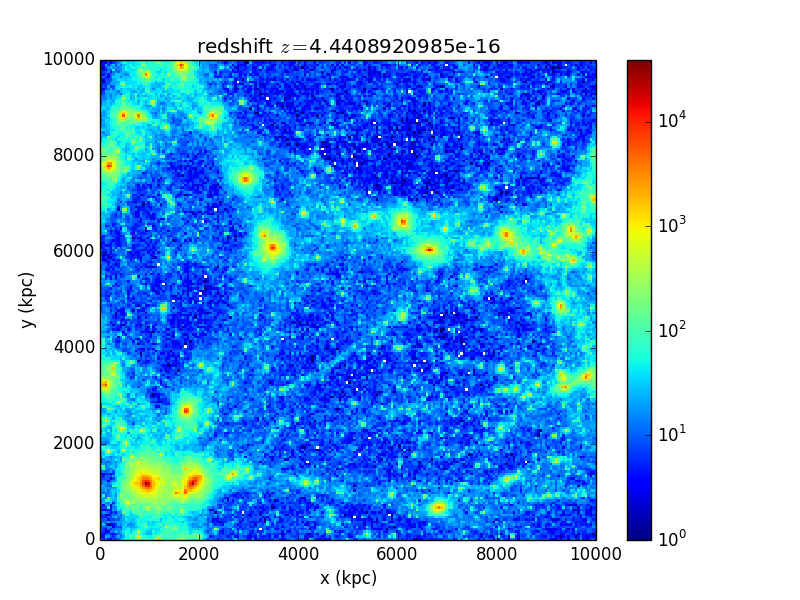
\includegraphics[width=1.0\linewidth]{img/Read_ics_1.png}
  \caption{High resolution}
  \label{fig:sub1}
\end{subfigure}%
\begin{subfigure}{.5\textwidth}
  \centering
  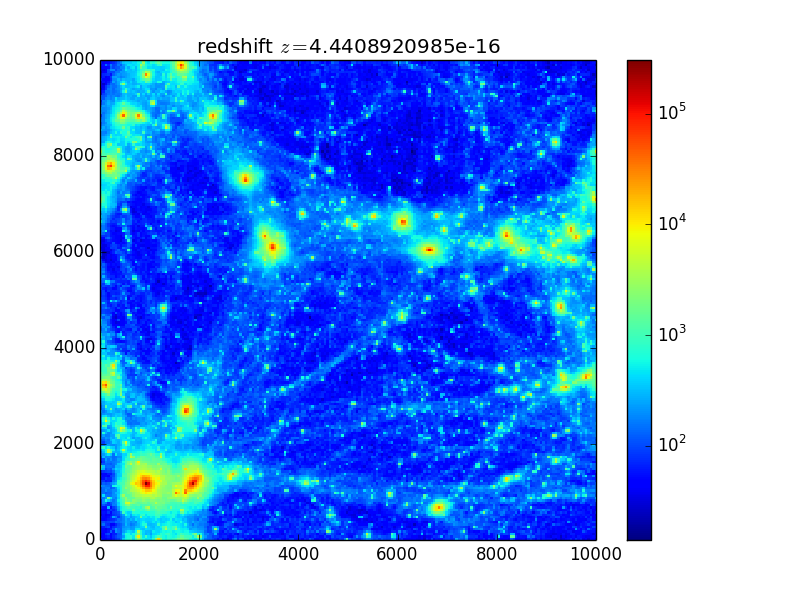
\includegraphics[width=1.0\linewidth]{img/Read_ICS_10MPC_1.png}
  \caption{Low resolution}
  \label{fig:sub2}
\end{subfigure}
\caption{Image of the 10 Megaparsec structure from the Gadget-2 simulation with G-perturbations. The most luminous clumps in the structure are galaxy cluster halos of dark matter.}
\label{fig:test}
\end{figure}

\begin{figure}
\centering
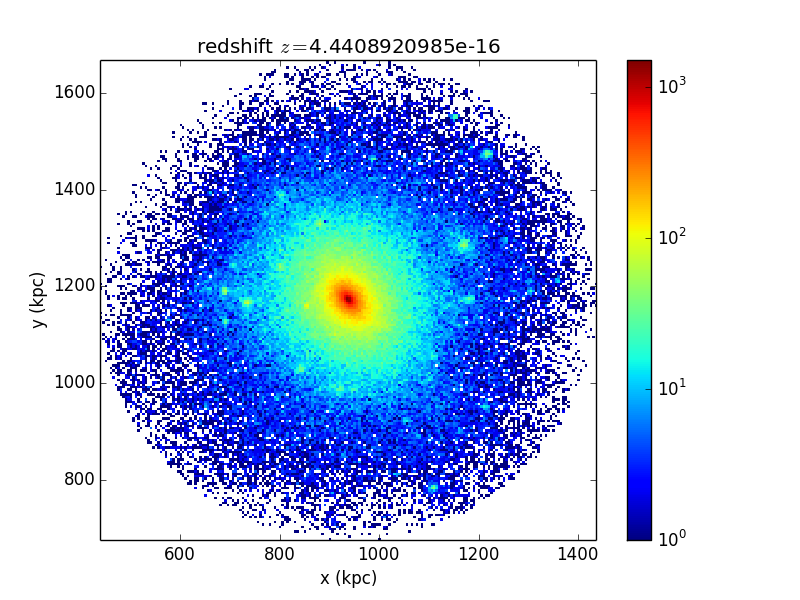
\includegraphics[width=1.0\linewidth]{img/Read_ics_2.png}
\caption{From the previous high resolution image of the 10 Mpc structure, 
the largest galaxy cluster halo of dark matter has been cut out to produce this image.}
\label{fig:test}
\end{figure}

\begin{figure}
\centering
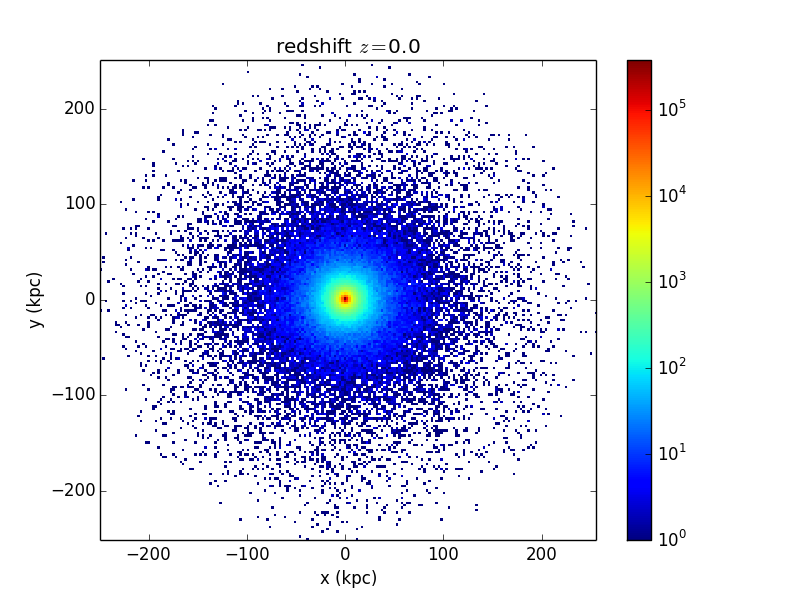
\includegraphics[width=1.0\linewidth]{img/Read_OG_IC_2.png}
\caption{Initial plot of G-perturbations with $ \beta = 0$ for a Hernquist structure (0G00\_IC\_000.hdf5).}
\label{fig:test}
\end{figure}

\begin{figure}
\centering
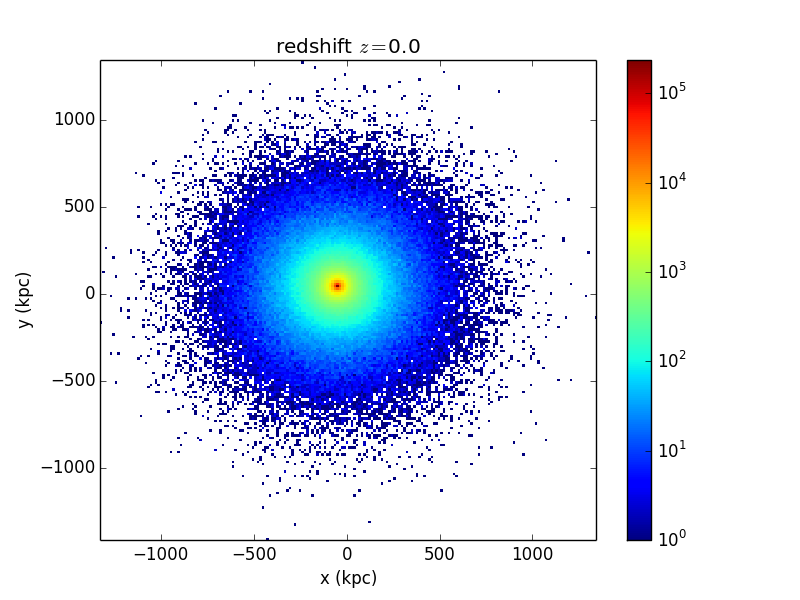
\includegraphics[width=1.0\linewidth]{img/Read_OG_Final_2.png}
\caption{Final plots of G-perturbations with $ \beta = 0$ for a Hernquist structure (0G20\_Final\_000.hdf5). Notice the structure has expanded significantly with respect to the initial structure.}
\label{fig:test}
\end{figure}

\begin{figure}
\centering
\begin{subfigure}{.5\textwidth}
  \centering
  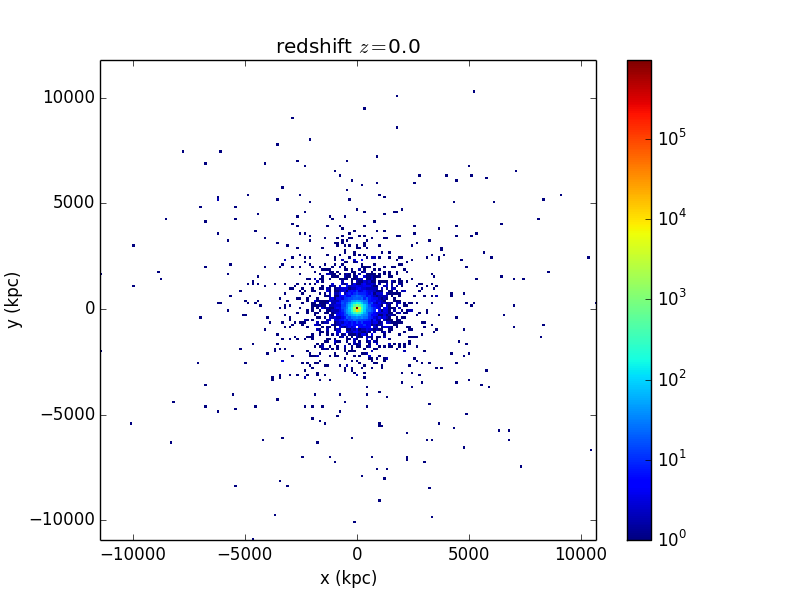
\includegraphics[width=1.0\linewidth]{img/Read_OMGOO_IC_1.png}
  \caption{The whole structure}
  \label{fig:sub1}
\end{subfigure}%
\begin{subfigure}{.5\textwidth}
  \centering
  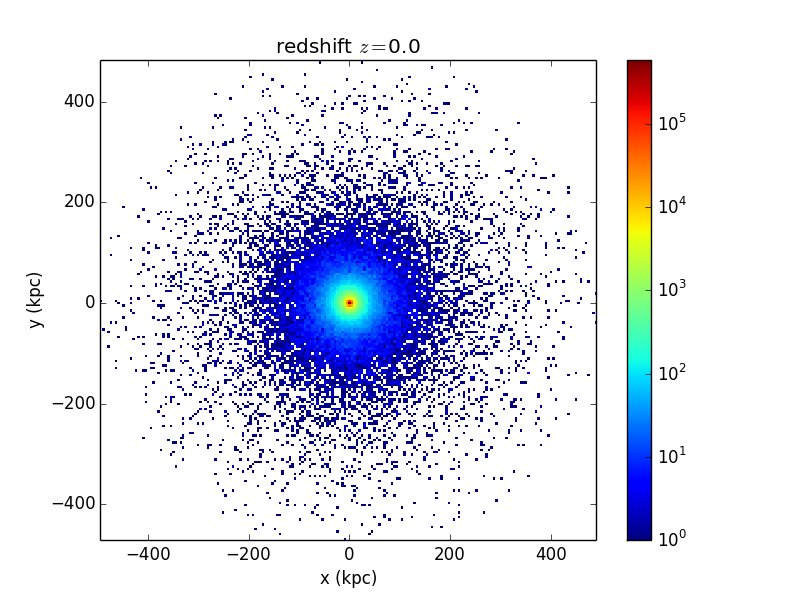
\includegraphics[width=1.0\linewidth]{img/Read_OMGOO_IC_2.png}
  \caption{Zoom-in on cluster}
  \label{fig:sub2}
\end{subfigure}
\caption{Initial plots of Osipkov-Merritt structure before G-perturbations.}
\label{fig:test}
\end{figure}

\begin{figure}
\centering
\begin{subfigure}{.5\textwidth}
  \centering
  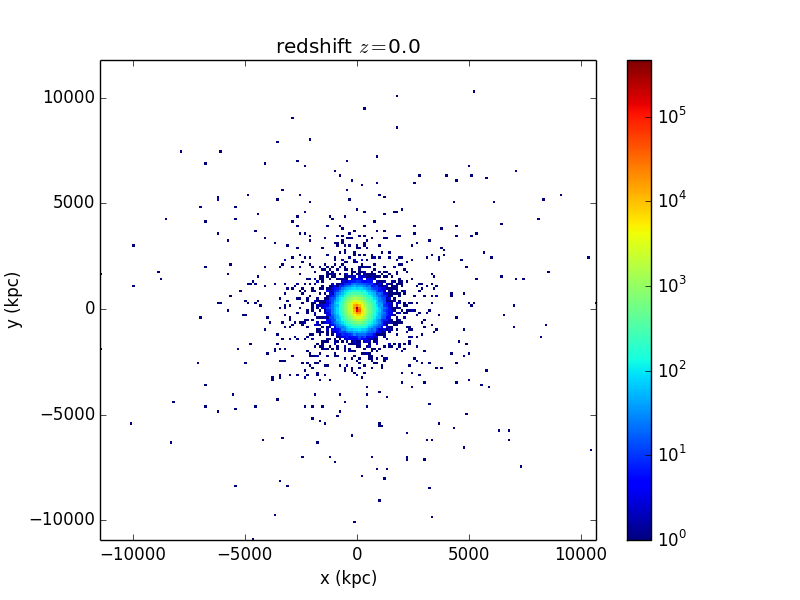
\includegraphics[width=1.0\linewidth]{img/Read_OMGOO_Final_1.png}
  \caption{The whole structure}
  \label{fig:sub1}
\end{subfigure}%
\begin{subfigure}{.5\textwidth}
  \centering
  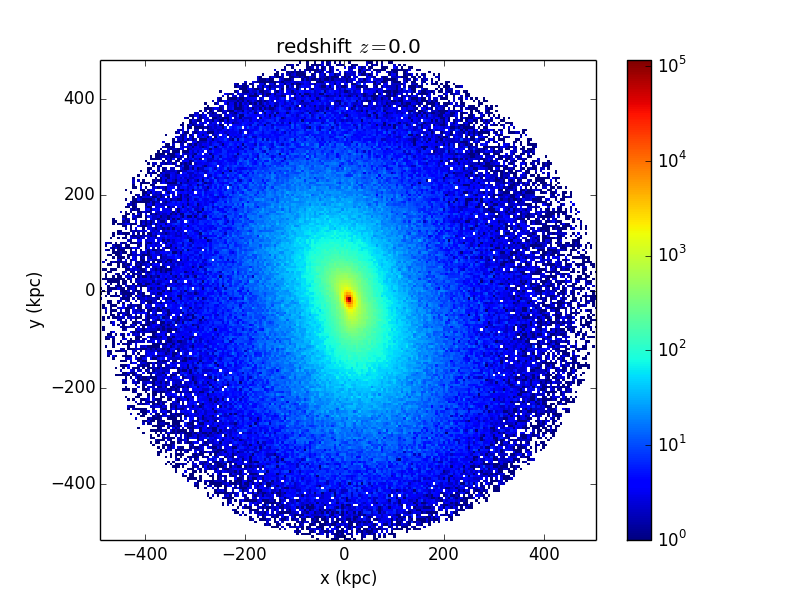
\includegraphics[width=1.0\linewidth]{img/Read_OMGOO_Final_2.png}
  \caption{Zoom-in on cluster}
  \label{fig:sub2}
\end{subfigure}
\caption{Final plots of Osipkov-Merritt structure after G-perturbations. Again we see how the structure has expanded significantly. }
\label{fig:test}
\end{figure}

\begin{figure}
\centering
\begin{subfigure}{.5\textwidth}
  \centering
  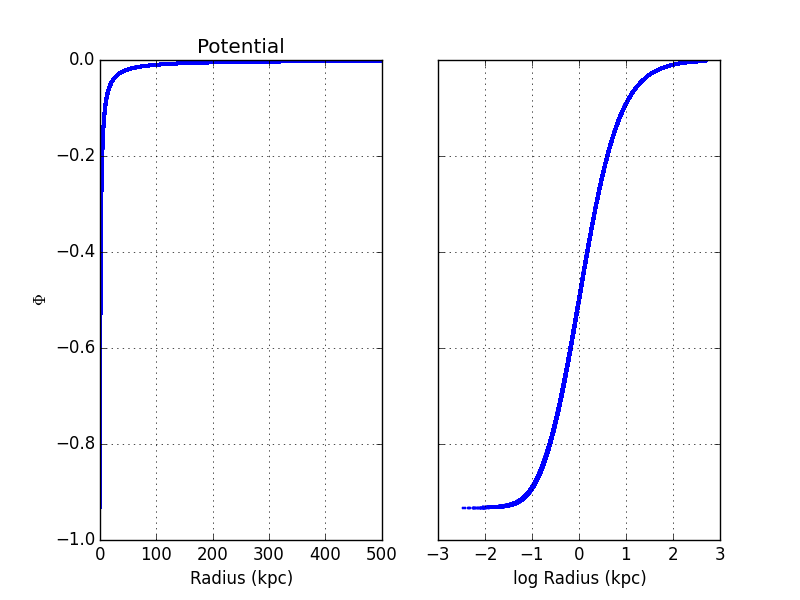
\includegraphics[width=1.0\linewidth]{img/Read_OMGOO_IC_3.png}
  \caption{Initially the central potential is close \\ to the value of -1}
  \label{fig:sub1}
\end{subfigure}%
\begin{subfigure}{.5\textwidth}
  \centering
  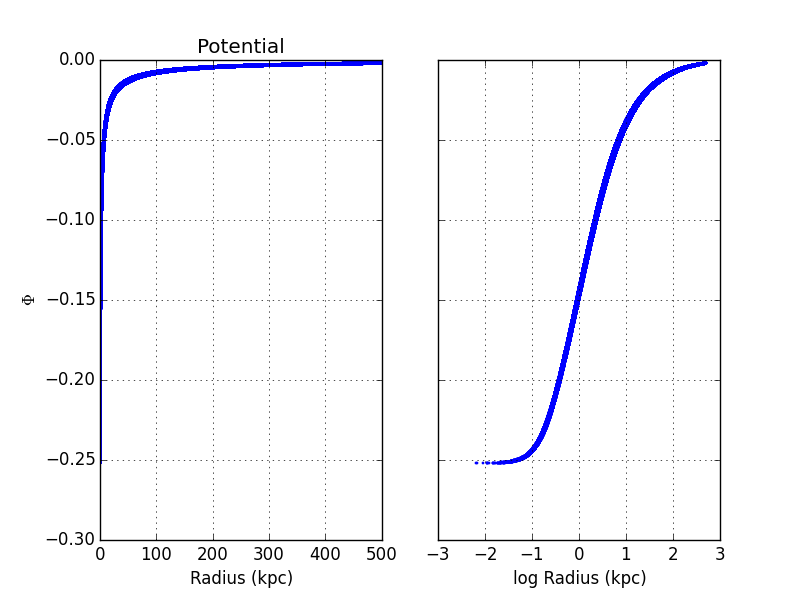
\includegraphics[width=1.0\linewidth]{img/Read_OMGOO_Final_3.png}
  \caption{Finally the central potential is seen in the semi-logarithmic plot to have a value of about \\ -0.25. }
  \label{fig:sub2}
\end{subfigure}
\caption{Gravitational potential for Osipkov-Merritt data. First subplot is $\Phi$ shown versus radius, whereas the second plot is against logarithmic radius, to resolve the central region in greater detail. The lessening of the central potential is to be expected since we already saw in a previous plot how the structure expands and therefore feels a numerically smaller central gravitational potential.}
\label{fig:test}
\end{figure}

\begin{figure}
\centering
\begin{subfigure}{.5\textwidth}
  \centering
  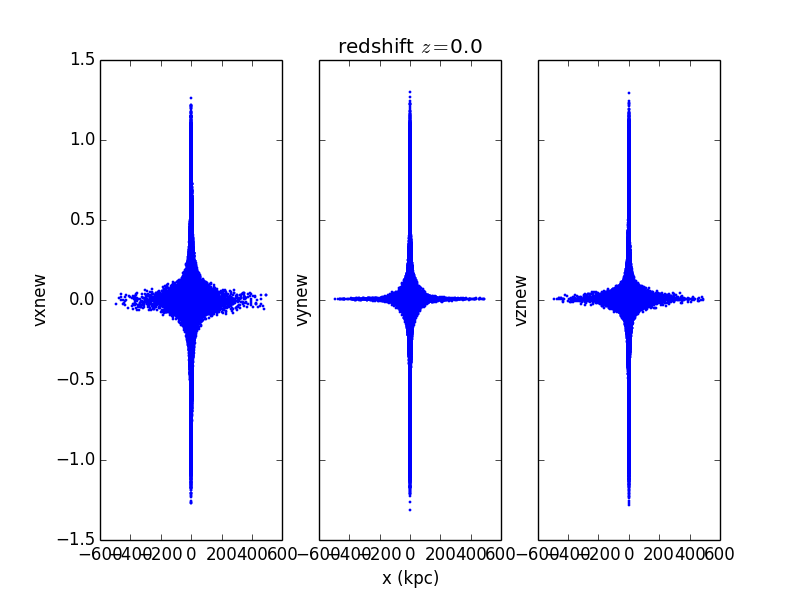
\includegraphics[width=1.0\linewidth]{img/Read_OMGOO_IC_5.png}
  \caption{Initially all velocities are almost identical}
  \label{fig:sub1}
\end{subfigure}%
\begin{subfigure}{.5\textwidth}
  \centering
  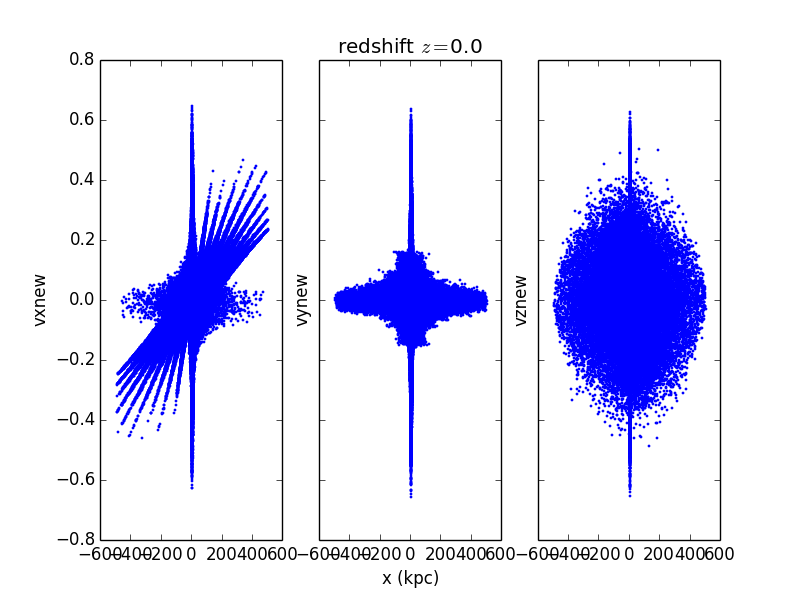
\includegraphics[width=1.0\linewidth]{img/Read_OMGOO_Final_5.png}
  \caption{The final picture is quite different. Now the velocities are completely different along each axis.}
  \label{fig:sub2}
\end{subfigure}
\caption{Velocities of particles , inside cluster of Osipkov-Merritt data, with respect to the clusters own velocity. From left to right we see particle velocities along the x, y and z-axis, all plotted as a function of the x-axis.}
\label{fig:test}
\end{figure}

\newpage
\begin{figure}[h!]
	\centering
		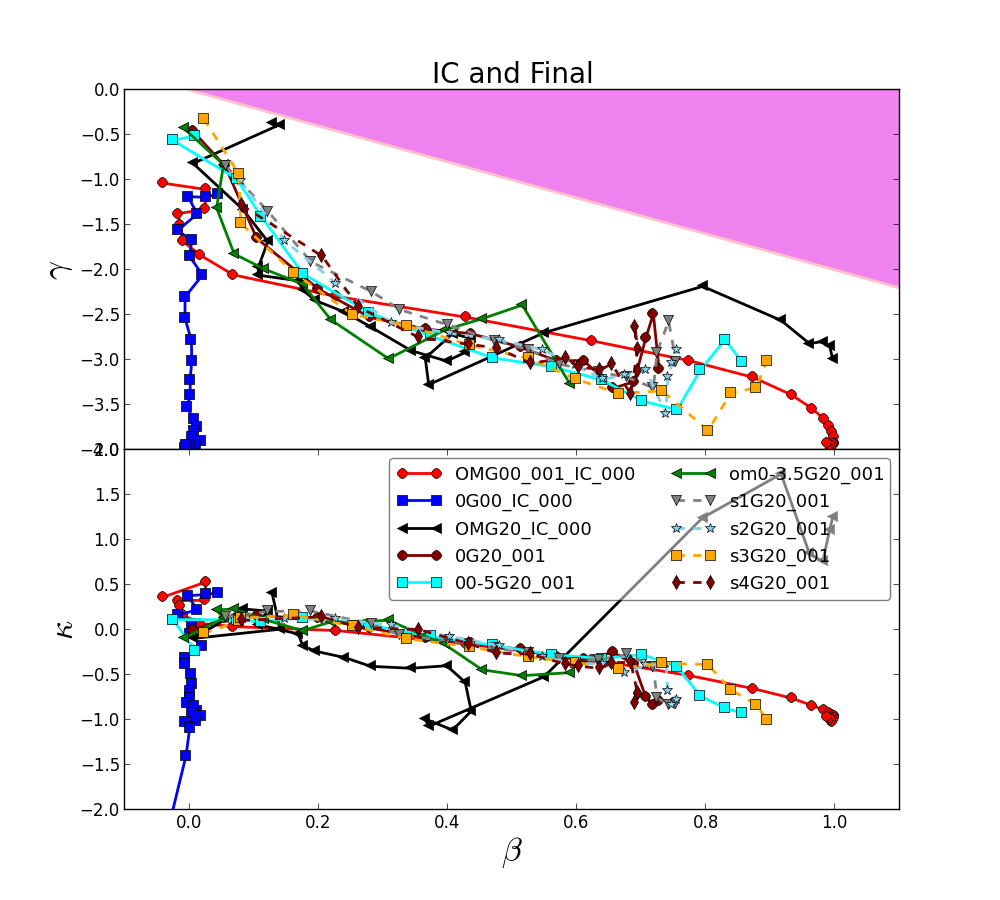
\includegraphics[width=1.0\linewidth]{img/Attractor_fig1.png}
		{\medskip\caption{\textsl{Now that the $\gamma$ ,$\kappa $ and $\beta$- profiles have been determined, the attractor in $(\gamma,\kappa,\beta)$-space can be created for all datasets. Notice how the upper right corner is always completely empty in the ($\beta$,$\gamma$)-plot. This is due to the constraint put by the inequality $ \beta < -\frac{\gamma}{2}$ (An \& Evans 2006).
\label{fig:Rv}}}}
\end{figure} 

\begin{figure}[h!]
	\centering
		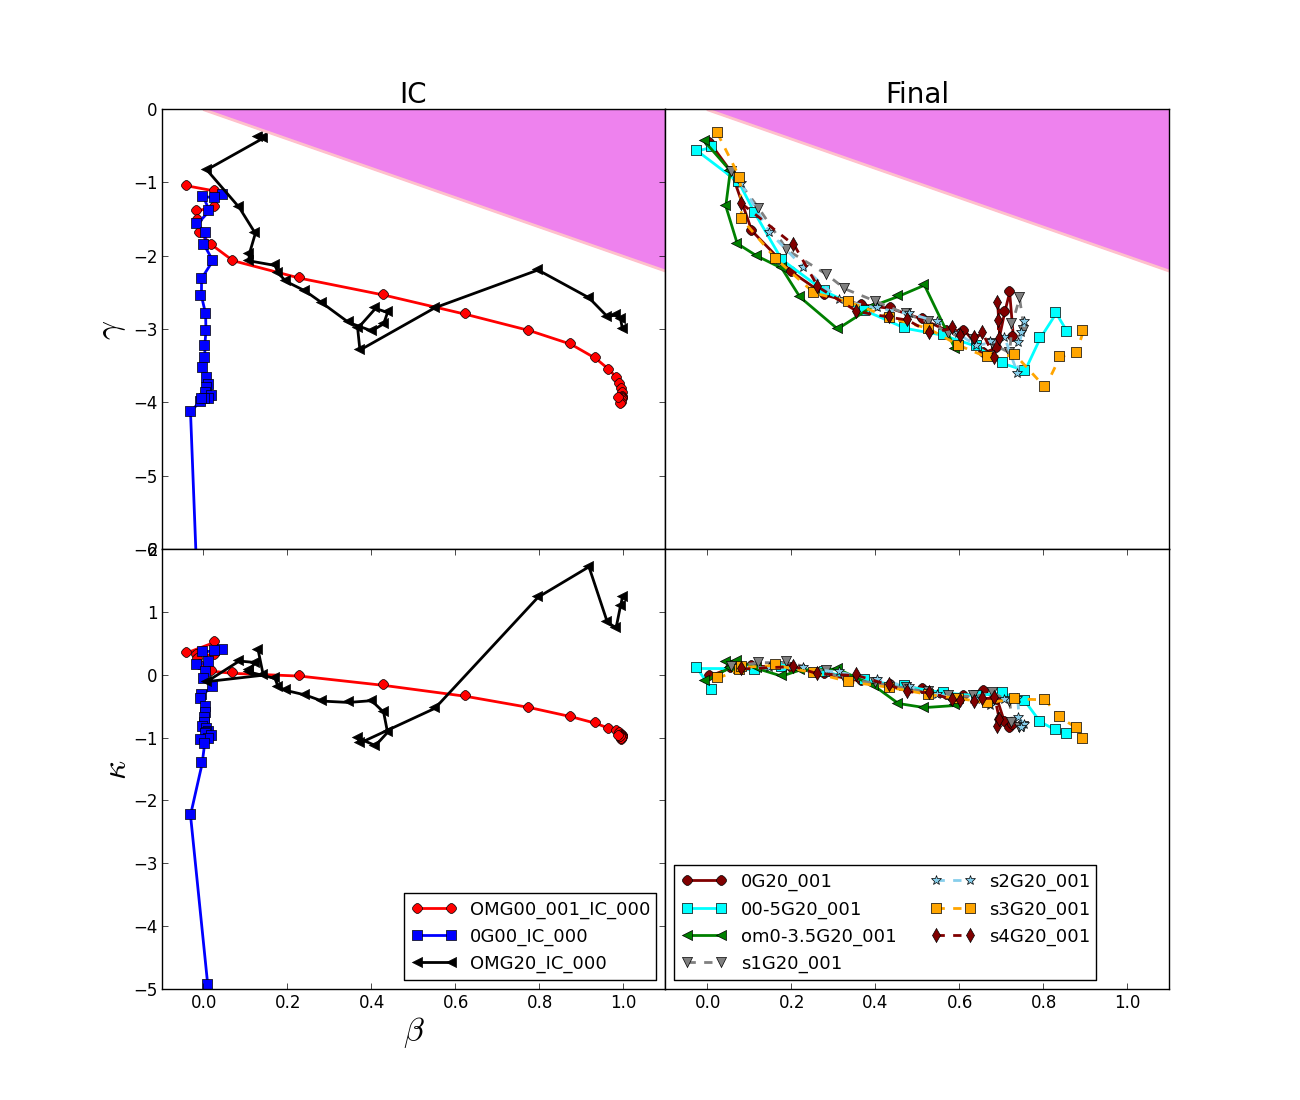
\includegraphics[width=1.0\linewidth]{img/Attractor_fig2.png}
		{\medskip\caption{\textsl{In the previous figure the IC and Final products had been overplotted. Here they can be seen independently.
\label{fig:Rv}}}}
\end{figure} 

\begin{figure}[h!]
	\centering
		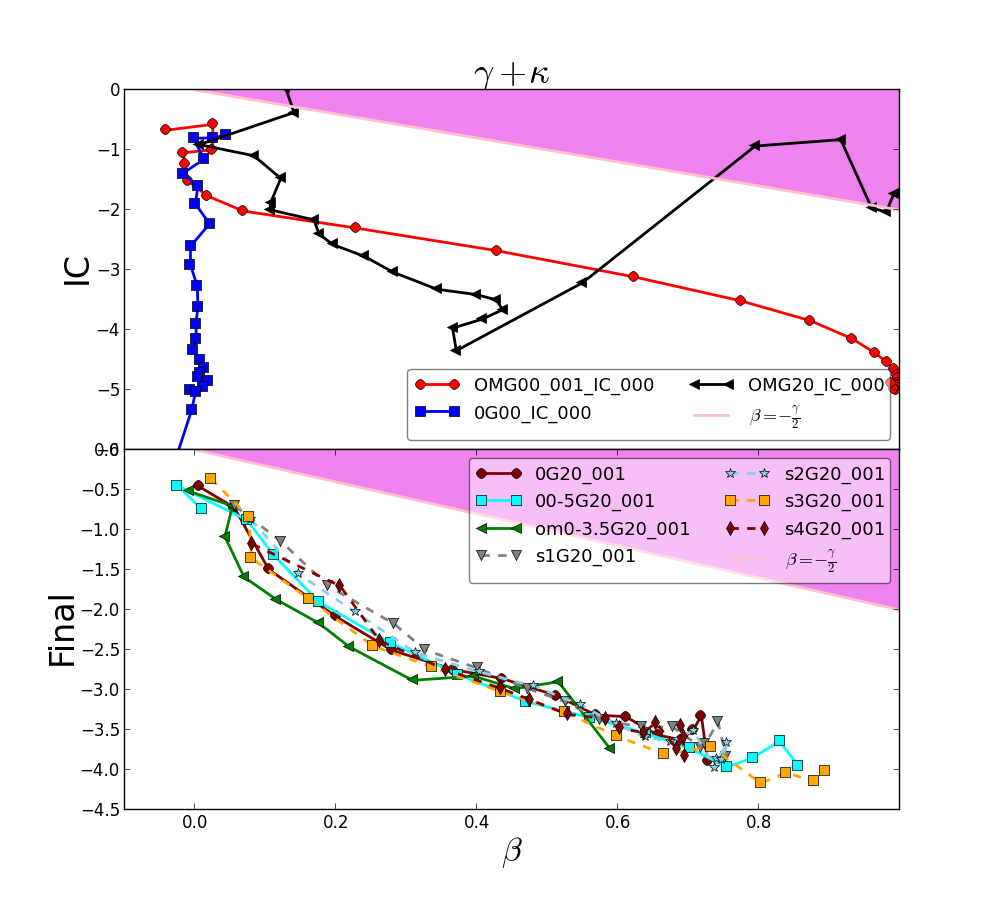
\includegraphics[width=1.0\linewidth]{img/Attractor_fig3.png}
		{\medskip\caption{\textsl{It is more clear to identify an attractor when $\gamma + \kappa$ is plotted vs. $\beta$, instead of splitting it up into two separate plots.
\label{fig:Rv}}}}
\end{figure} 

\begin{figure}[h!]
	\centering
		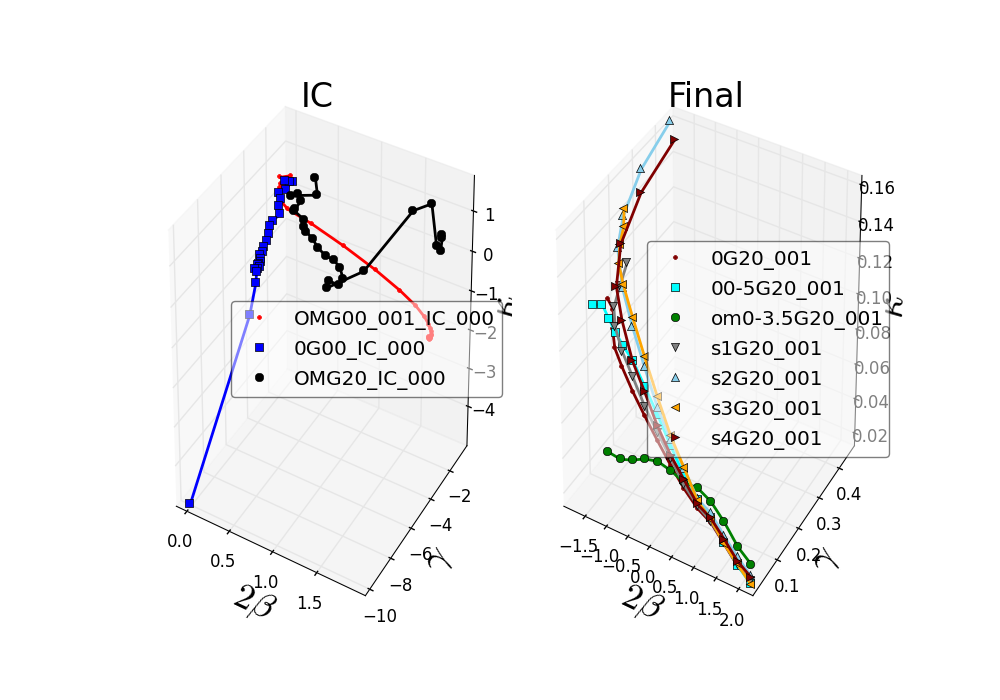
\includegraphics[width=1.0\linewidth]{img/Attractor_3D.png}
		{\medskip\caption{\textsl{3D view of attractor.
\label{fig:Rv}}}}
\end{figure} 

\begin{figure}[h!]
	\centering
		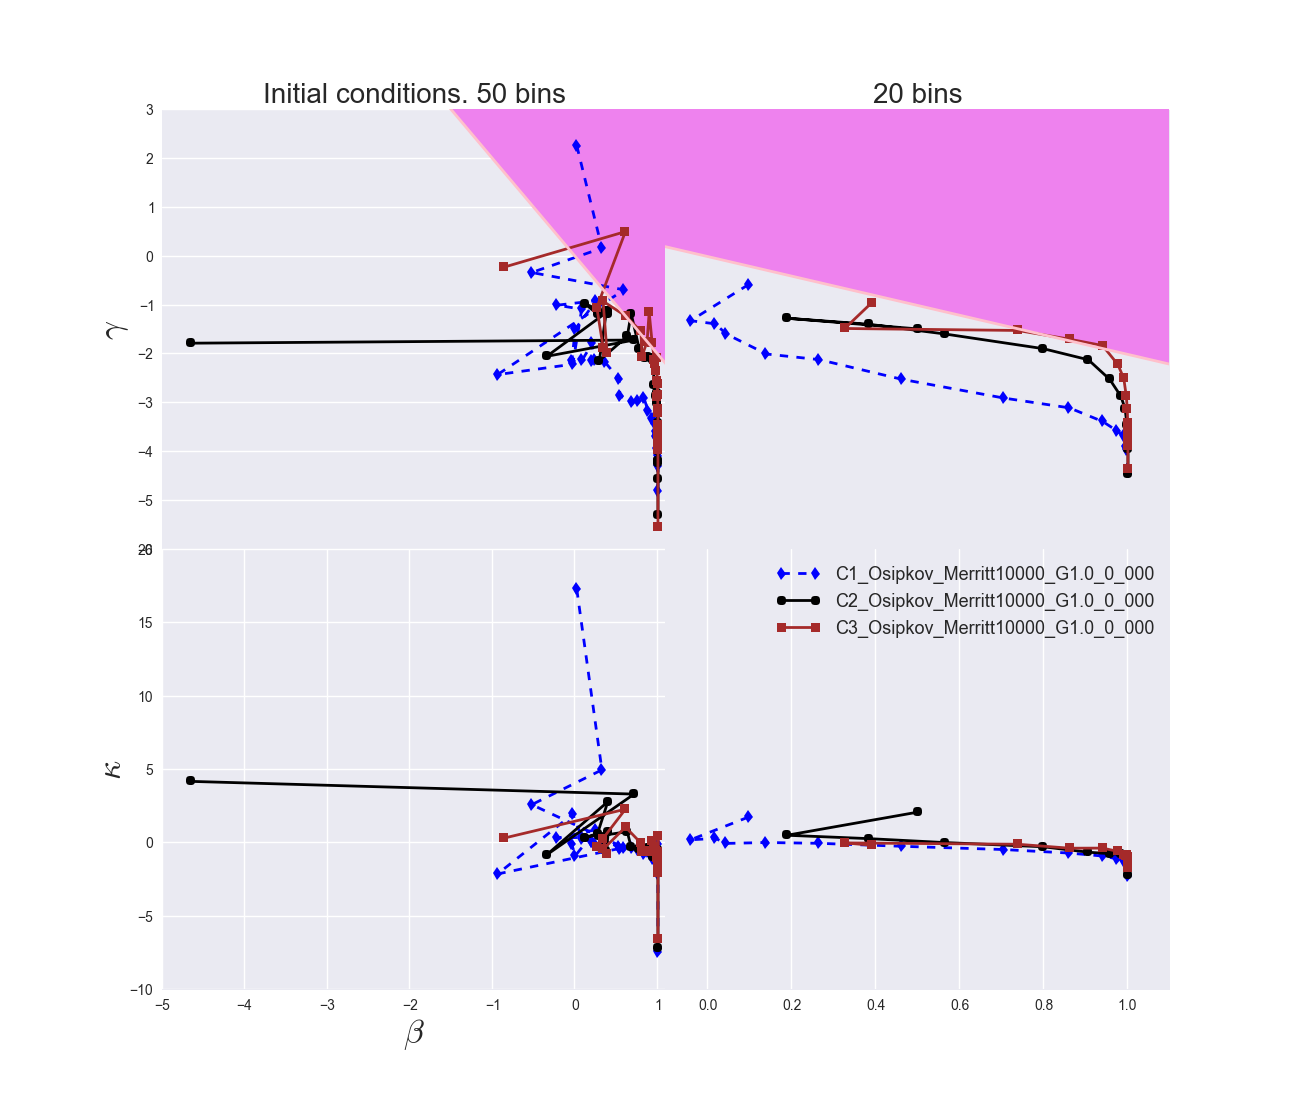
\includegraphics[width=1.0\linewidth]{img/C1C2C3_beta_gamma_kappa.png}
		{\medskip\caption{\textsl{$\gamma$ vs. $\beta$ and $\kappa$ vs. $\beta$ for 50 and 20 radial bins is here shown for the ICs of sims. $C_1$, $C_2$ and $C_3$ which each hold a total number of $N = 10^4$ particles. $R_{limit} = 5 \cdot 10^2$.
50 bins introduces random scatter due to bad resolution and is not physical.
\label{fig:Rv}}}}
\end{figure} 

\begin{figure}[h!]
	\centering
		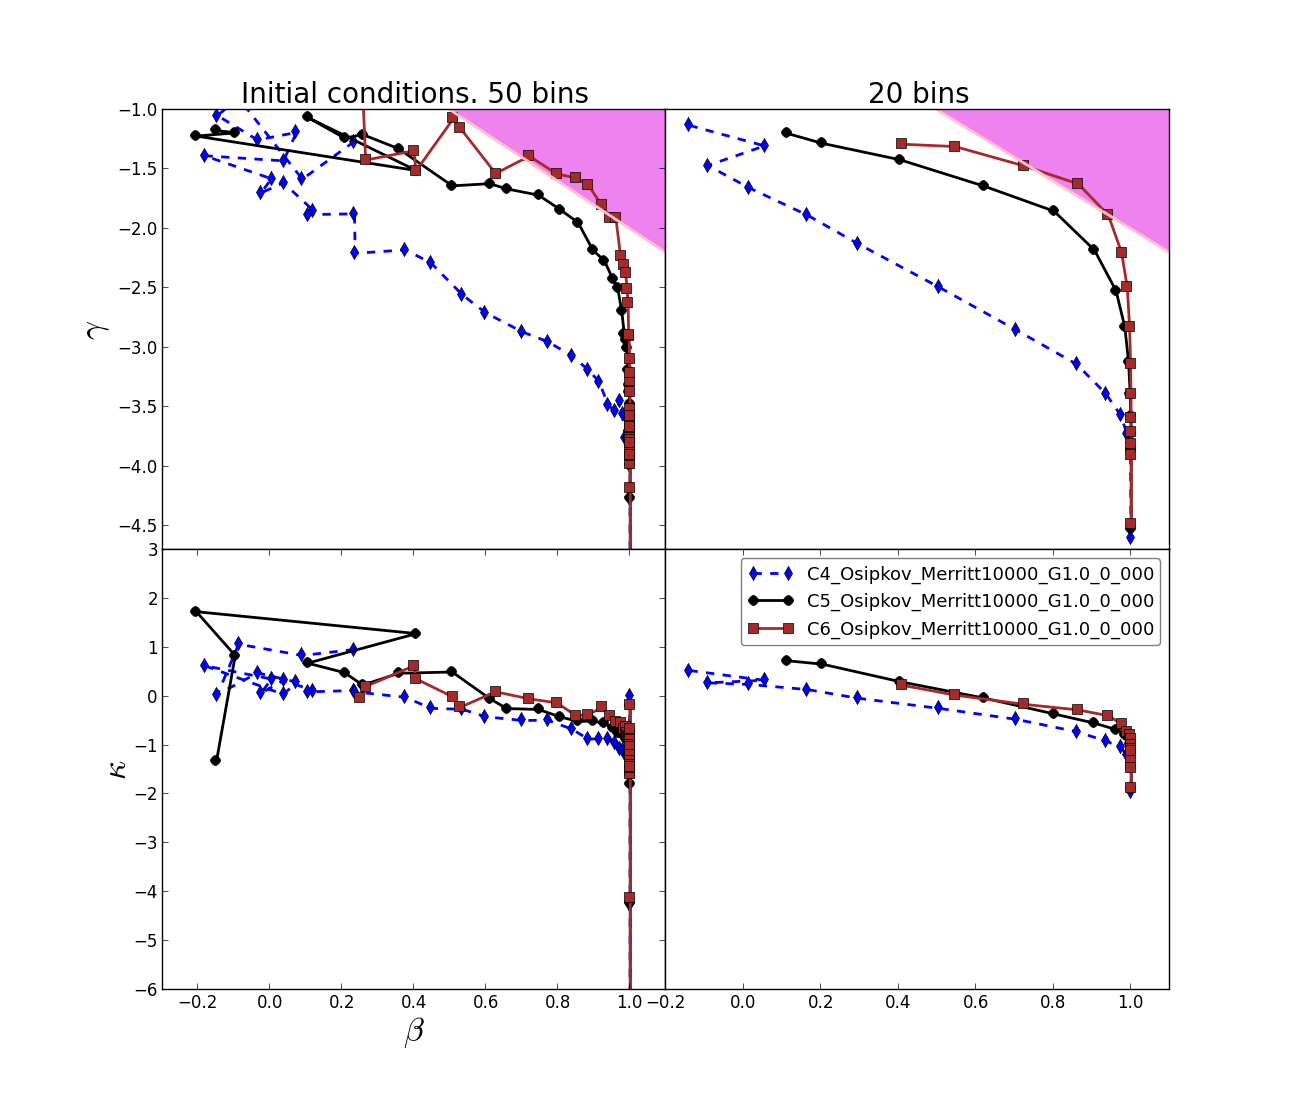
\includegraphics[width=1.0\linewidth]{img/C4C5C6_beta_gamma_kappa.png}
		{\medskip\caption{\textsl{$\gamma$ vs. $\beta$ and $\kappa$ vs. $\beta$ for 50 and 20 radial bins is here shown for the IC´s of SIMS $C_4$, $C_5$ and $C_6$ which each hold a total number of $N = 10^5$ particles. $R_{limit} = 5 \cdot 10^2$. 50 bins introduces random scatter due to bad resolution and is not physical.
\label{fig:Rv}}}}
\end{figure} 

\begin{figure}[h!]
	\centering
		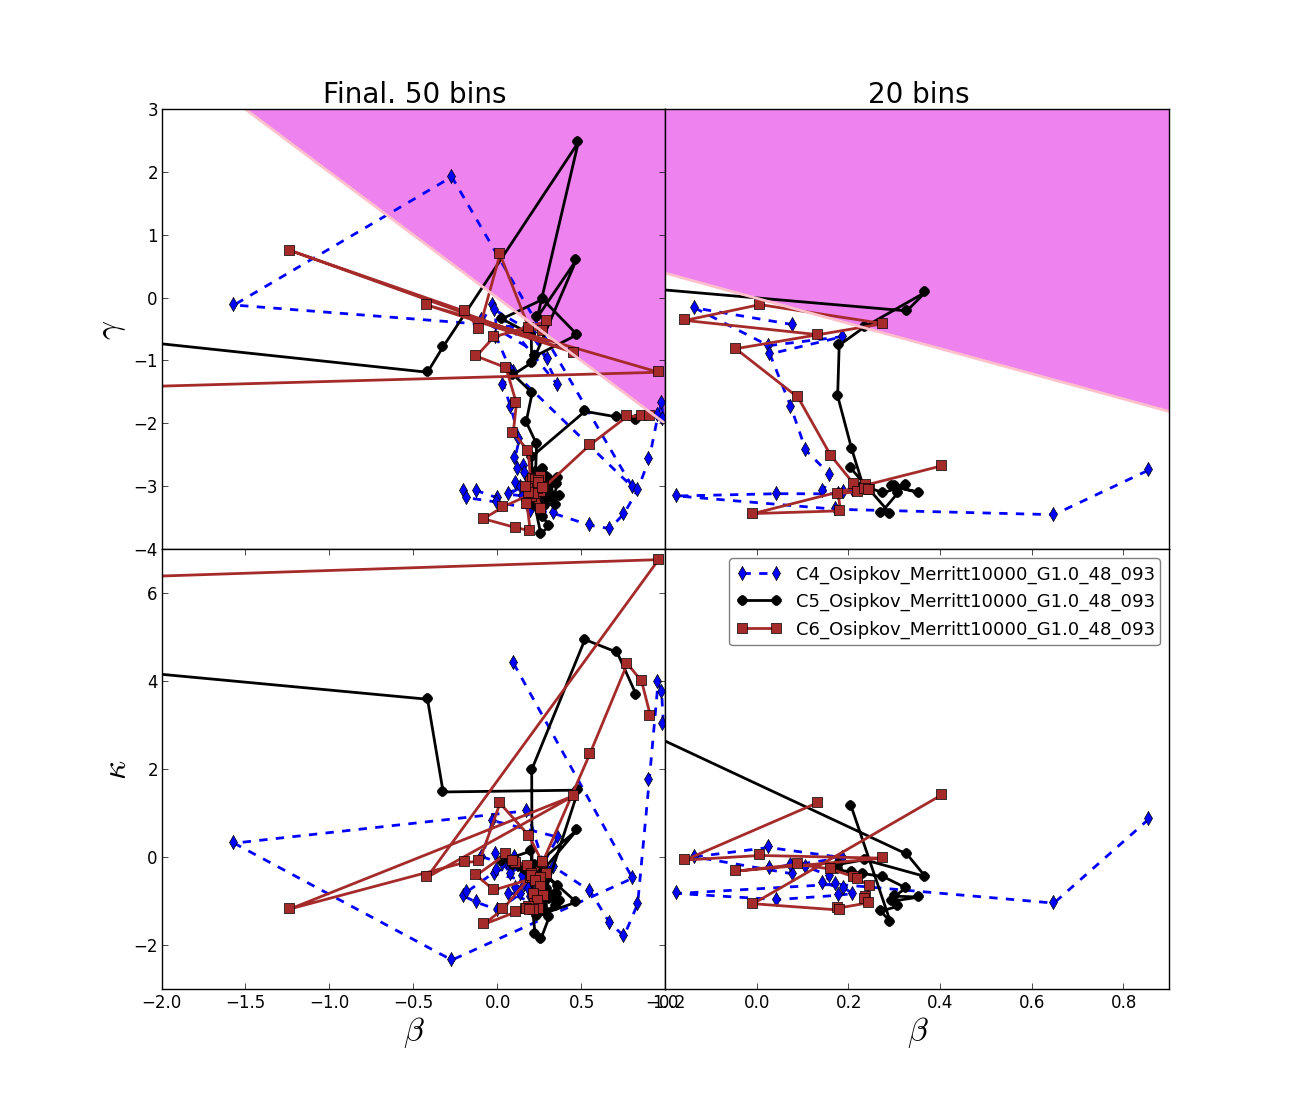
\includegraphics[width=1.0\linewidth]{img/C4C5C6_beta_gamma_kappa_Final.png}
		{\medskip\caption{\textsl{$\gamma$ vs. $\beta$ and $\kappa$ vs. $\beta$ for 50 and 20 radial bins is here shown for the final products of sims. $C_4$, $C_5$ and $C_6$. $R_{limit} = 5 \cdot 10^2$. 50 bins introduces random scatter due to bad resolution and is not physical.
\label{fig:Rv}}}}
\end{figure} 

\begin{figure}[h!]
	\centering
		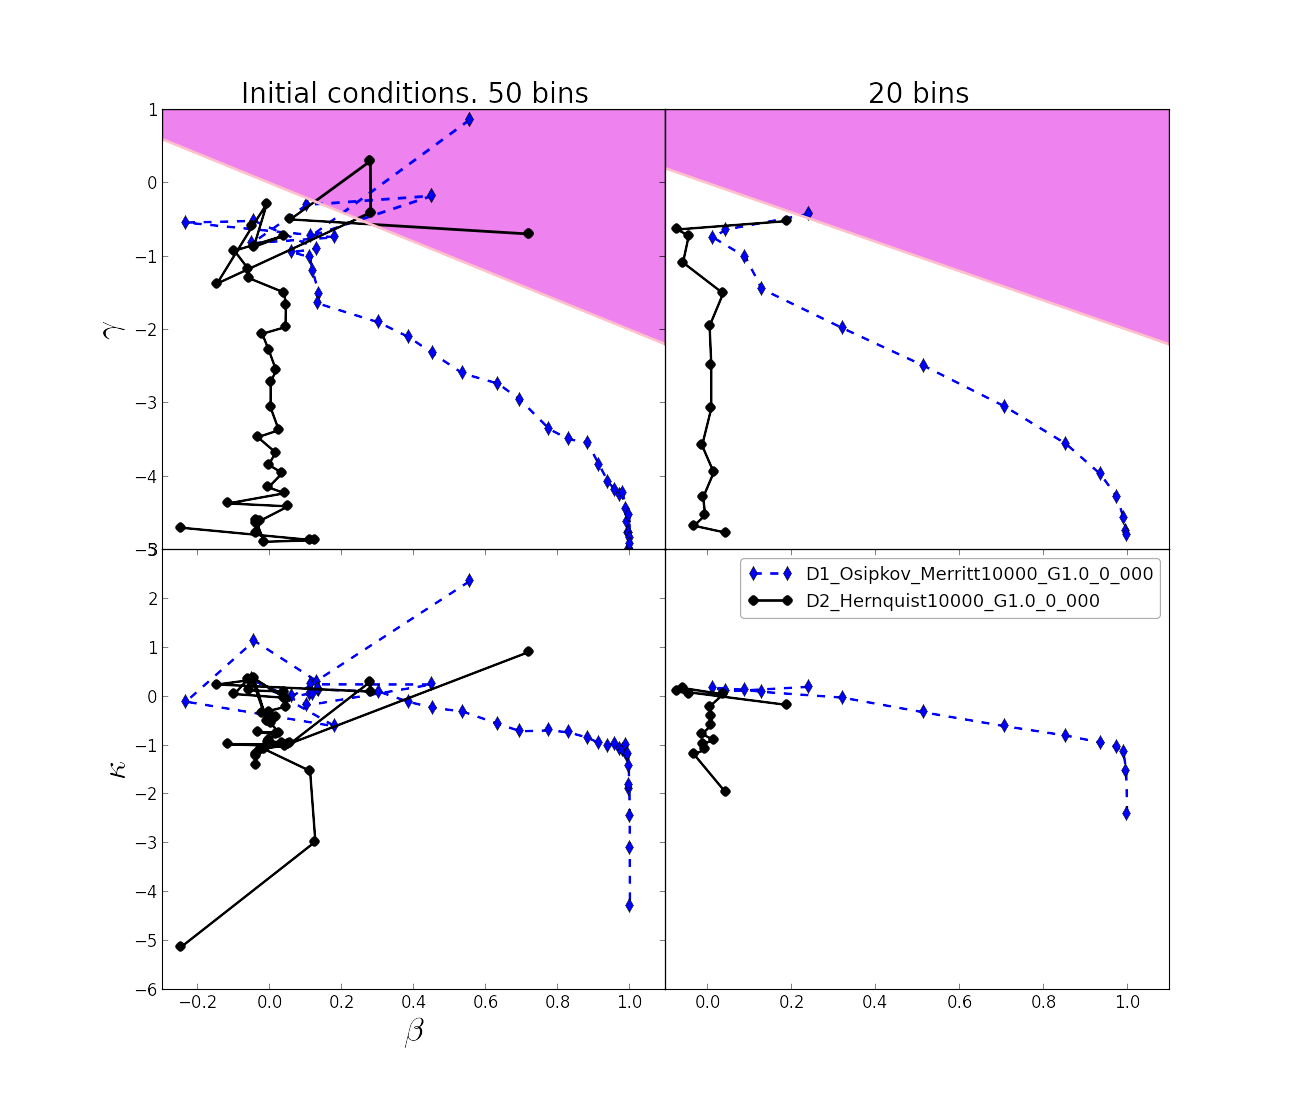
\includegraphics[width=1.0\linewidth]{img/D1D2_beta_gamma_kappa.png}
		{\medskip\caption{\textsl{$\gamma$ vs. $\beta$ and $\kappa$ vs. $\beta$ for 50 and 20 radial bins is here shown for the IC´s of sims. $D_1$ and $D_2$ which both hold a total number of $N = 10^5$ particles. $R_{limit} = 5 \cdot 10^2$. 50 bins introduces random scatter due to bad resolution and is not physical.
\label{fig:Rv}}}}
\end{figure} 

\begin{figure}[h!]
	\centering
		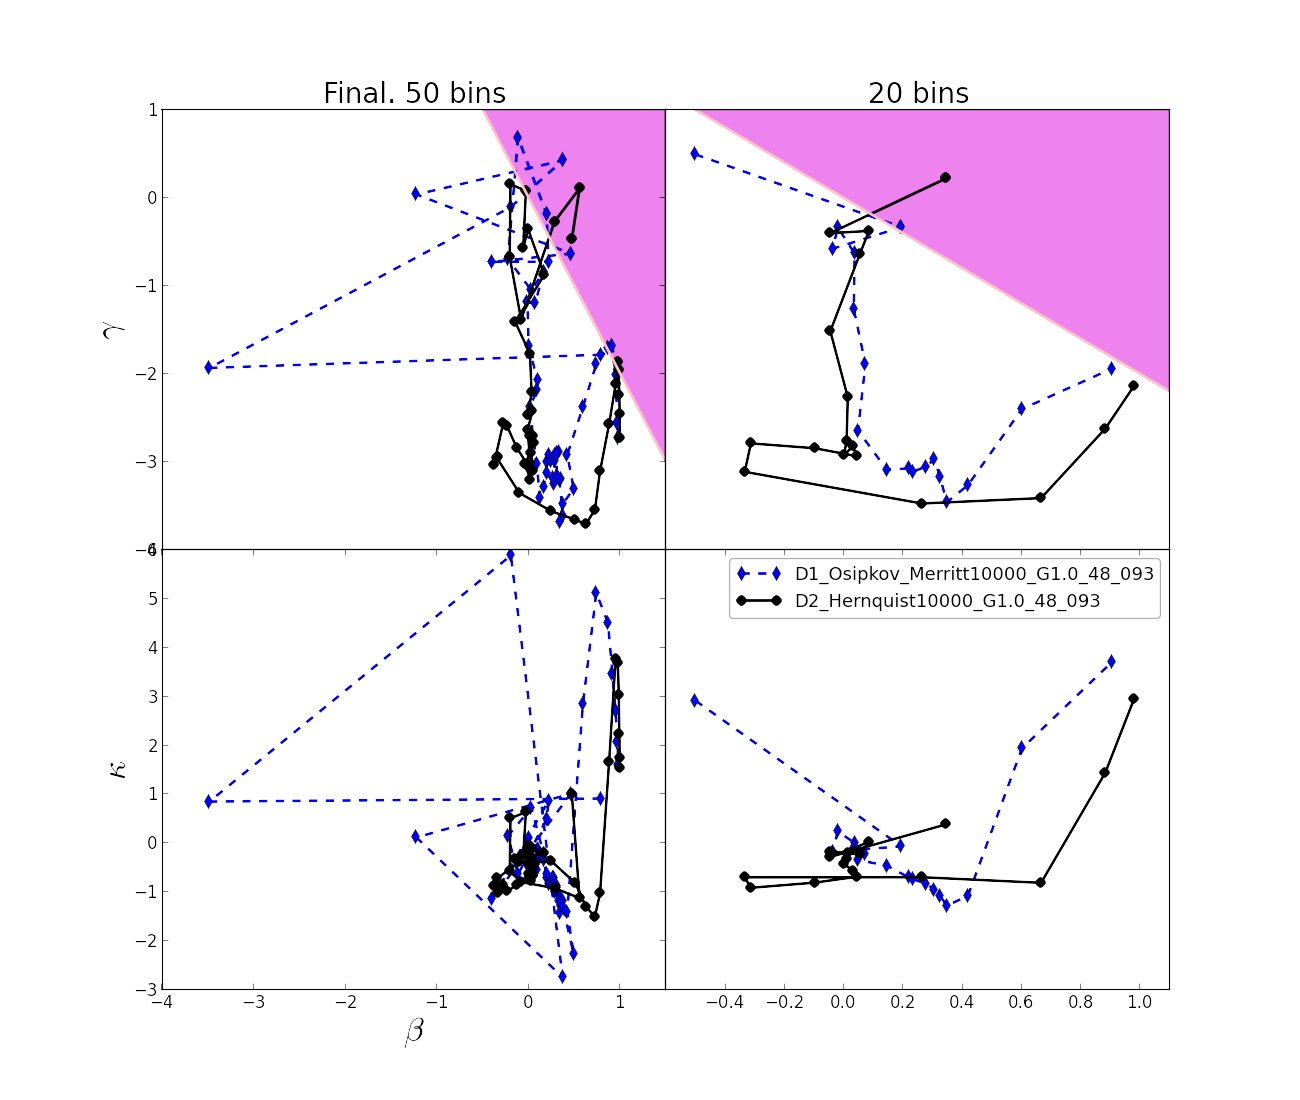
\includegraphics[width=1.0\linewidth]{img/D1D2_beta_gamma_kappa_Final.png}
		{\medskip\caption{\textsl{$\gamma$ vs. $\beta$ and $\kappa$ vs. $\beta$ for 50 and 20 radial bins is here shown for the final products of sims. $D_1$ and $D_2$. $R_{limit} = 5 \cdot 10^2$. 50 bins introduces random scatter due to bad resolution and is not physical.
\label{fig:Rv}}}}
\end{figure} 

\begin{figure}[h!]
	\centering
		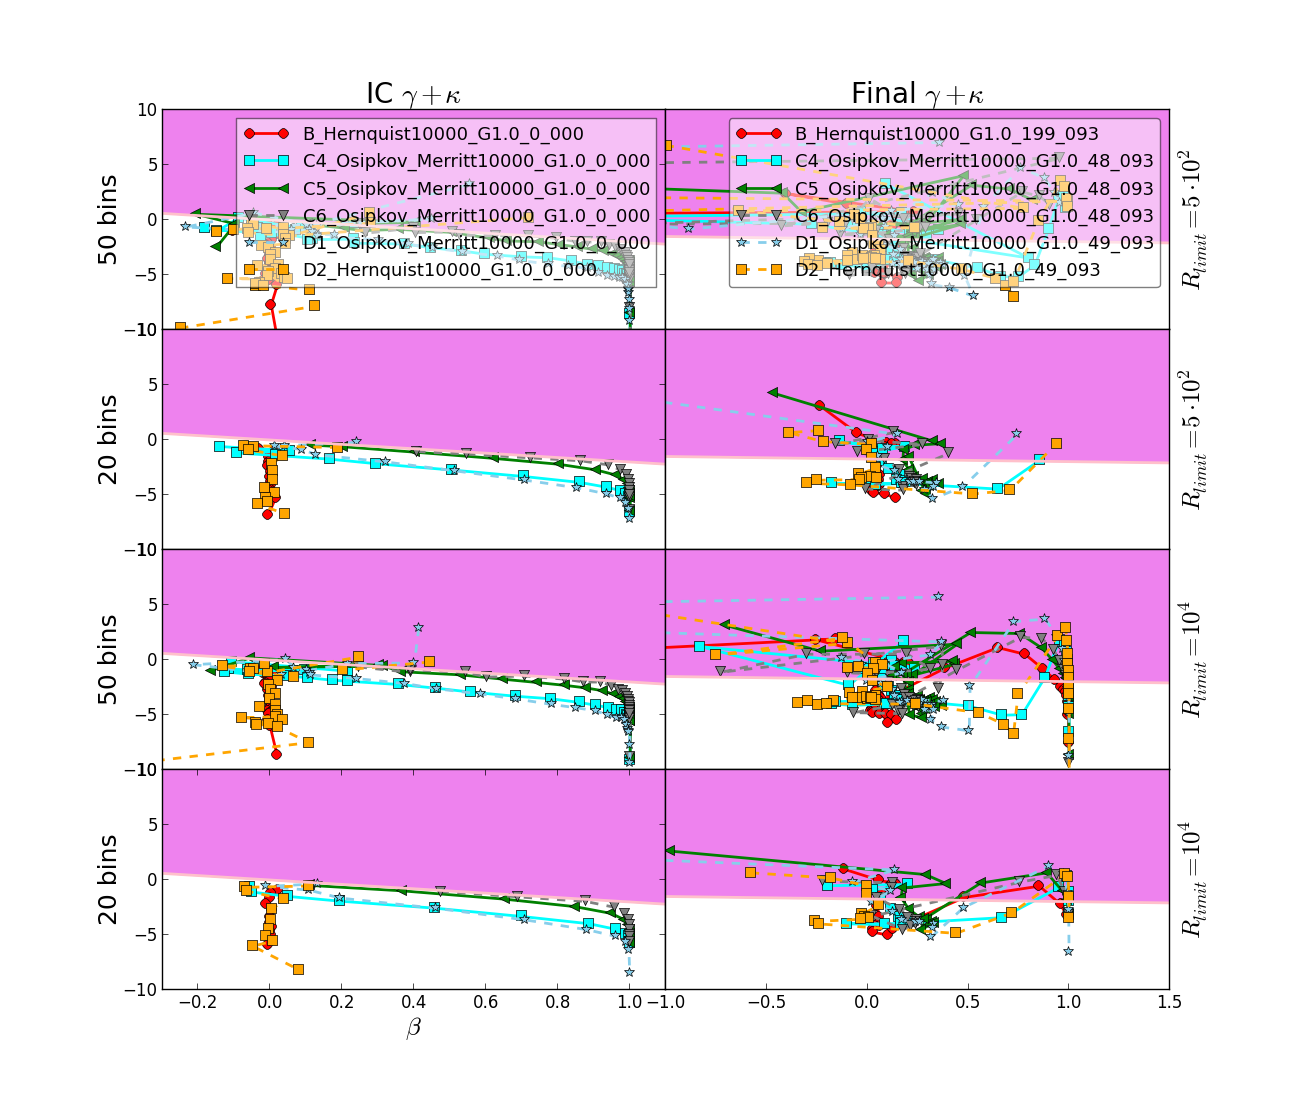
\includegraphics[width=1.0\linewidth]{img/Attractor_fig4.png}
		{\medskip\caption{\textsl{$\gamma + \kappa$ vs. $\beta$ for IC and Final of SIMS B, 
$C_4$, $C_5$, $C_6$, $D_1$ and $D_2$. For the upper four subplots $R_{limit} = 5 \cdot 10^2$, and for the lower four subplots $R_{limit} = 10^4$. Shown for both 20 and 50 radial bins.
\label{fig:Rv}}}}
\end{figure} 

\begin{figure}[h!]
	\centering
		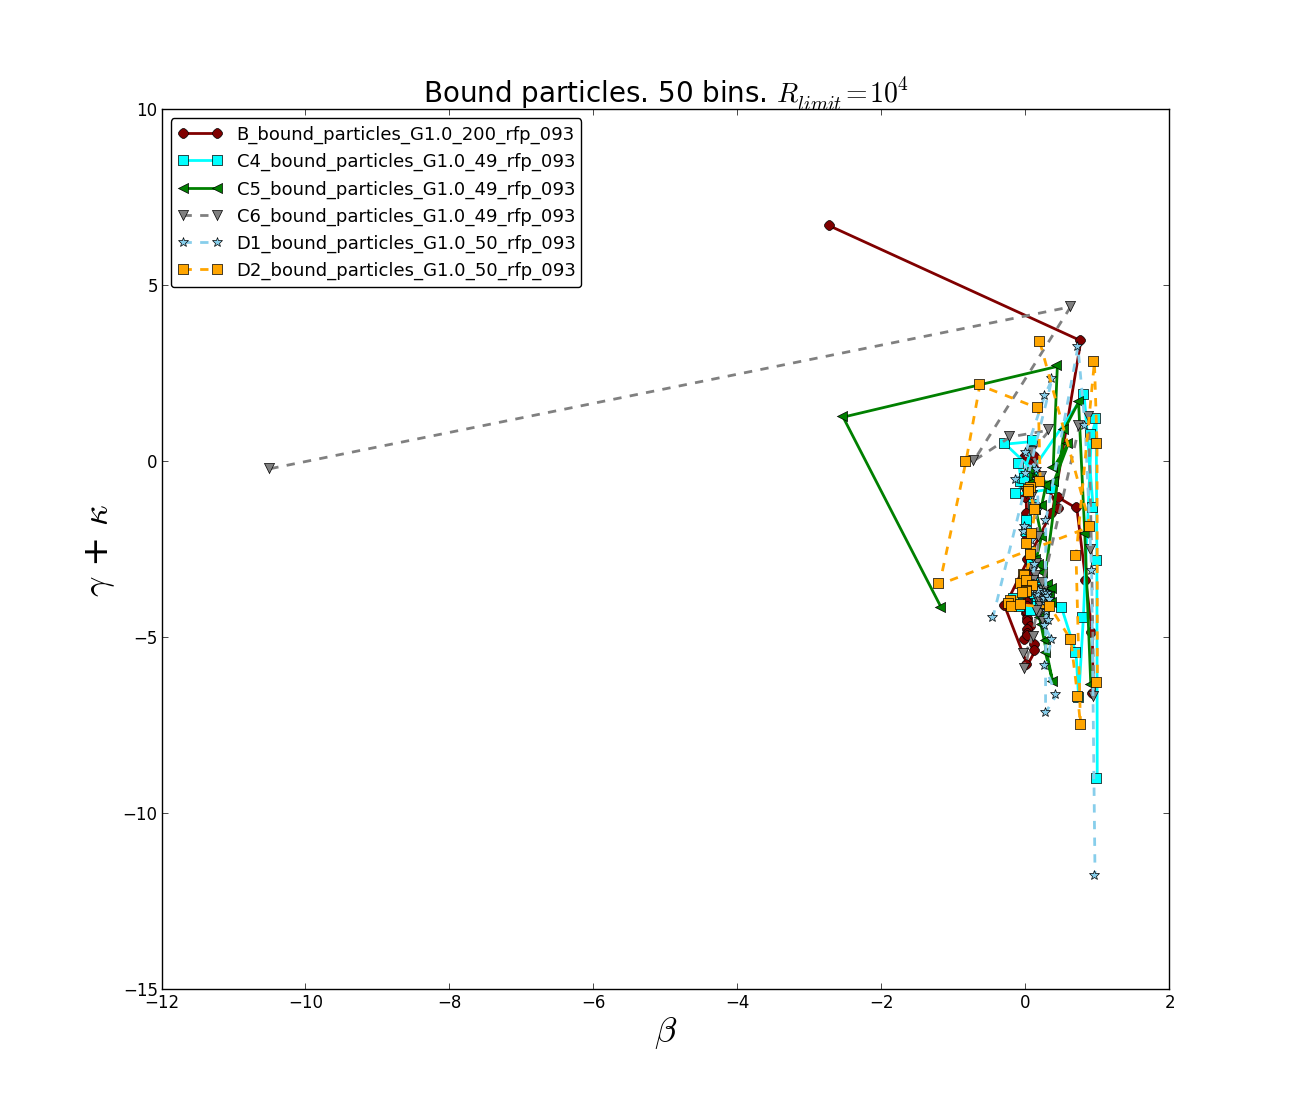
\includegraphics[width=1.0\linewidth]{img/Attractor_fig5.png}
		{\medskip\caption{\textsl{$\gamma + \kappa$ vs. $\beta$ for Final of SIMS B, 
$C_4$, $C_5$, $C_6$, $D_1$ and $D_2$ where all gravitationally unbound particles have been removed and the structures have had more time to equilibrate. $R_{limit} = 10^4$. 50 radial bins.
\label{fig:Rv}}}}
\end{figure} 

\subsection{Line-of-sight}

\subsection{Removing gravitationally unbound particles from structures}
To see the equilibrated structures from the final products more clearly, it is beneficial to remove the unbound particles which have escaped the gravitational potential of all the other particles. The total energy being positive is the condition which has to be met, in order to identify a free particle. This leads to the inequality $E_{tot} > 0 \rightarrow \Phi + \frac{1}{2}v^2 > 0$, where $\Phi$ is the gravitational potential of all the other particles and v is the speed of the particle under investigation. It is computed as $v = \sqrt{v_x^2+v_y^2+v_z^2}$. In practice this has been solved by writing all the bound particles (where $\Phi + \frac{1}{2}v^2 <= 0$) into a new HDF5 file, as deleting data inside a HDF5 file is rather complicated (commands such as HDF5DELETE does exist, and one could use this to destroy the link in the file to the data, after which the non-broken links can be saved in a new file, but that would be a messy solution). The new data is then inspected with the program HDFview to make sure the new file contain the right particles. The following table show the number of free and bound particles for final products of different SIMS:
\begin{table}[h]
\centering
\begin{tabular}{|c|c|c|c|c|c|c|}
\hline
         &     $B$    &    $C_4$  & $C_5$     & $C_6$     &  $D_1$    & $D_2$     \\ \hline
 File    & 199$\_$093 & 48$\_$093 & 48$\_$093 & 48$\_$093 & 49$\_$093 & 49$\_$093 \\ \hline
 N       &   $10^6$   &  $10^5$   & $10^5$    &  $10^5$   & $10^5$    & $10^5$  \\ \hline
 Bound   &   959845   &  58865    & 58917     &  58386    & 59340     & 66039  \\ \hline
 Unbound &   40155    &  41135    & 41083     &  41614    & 40660     & 33961  \\ \hline
\end{tabular}
\caption{From top to bottom: structure name, file number, total number of particles (N), number of bound particles and finally number of unbound particles. For all these files $G=1$.}
\end{table}
The bound particles from these simulations final products are thus saved into new files which are further simulated with GADGET-2 while G is kept equal to one for all these new files and they are all run for TimeMax = 2300. This result in the following files being created:
\begin{table}[h]
\centering
\begin{tabular}{|c|c|c|c|c|c|c|}
\hline
     &   $B$       &    $C_4$    &    $C_5$    &    $C_6$    &   $D_1$     &   $D_2$    \\ \hline
 N   &   959845    &    58865    &    58917    &    58386    &   59340     &   66039    \\ \hline
 Run No.       &   200       &     49      &     49      &      49     &     50      &     50     \\ \hline
\end{tabular}
\caption{From top to bottom: structure name, total number of particles N (Notice all gravitationally unbound particles have been removed), and finally number of the run is given. For all these files $G=1$.}
\end{table}

\begin{figure}
\centering
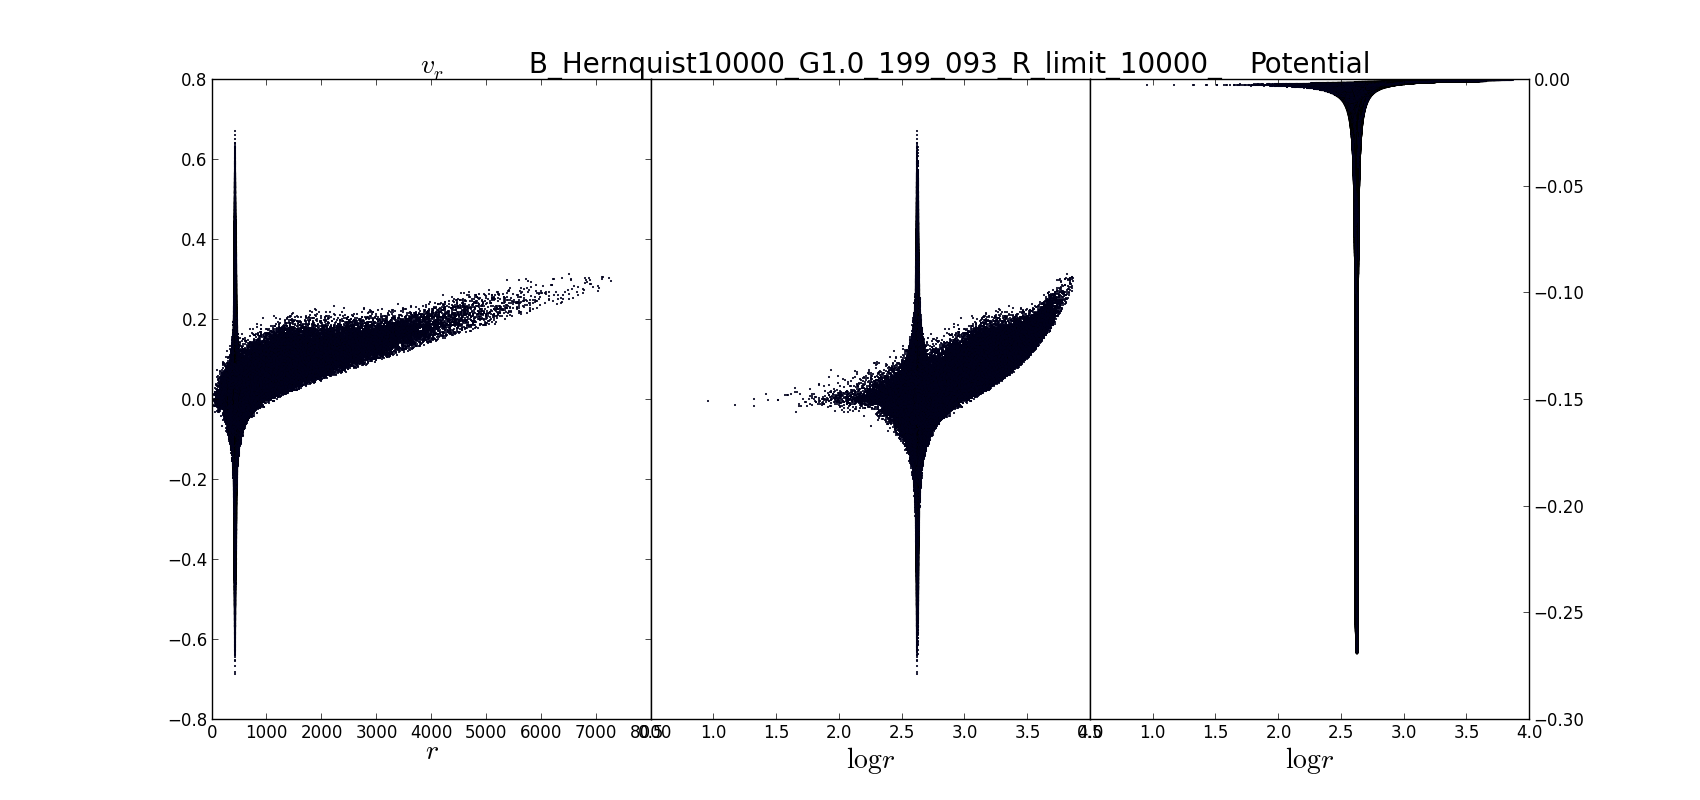
\includegraphics[width=1.0\linewidth]{img/B_final_vr_V_panel.png}
\caption{Final product of SIM B which have a total of $N = 10^6$ particles. Radial velocity vs. radius and logarithmic radius respectively. Gravitational potential vs. logarithmic radius.}
\label{fig:test}
\end{figure}

\begin{figure}
\centering
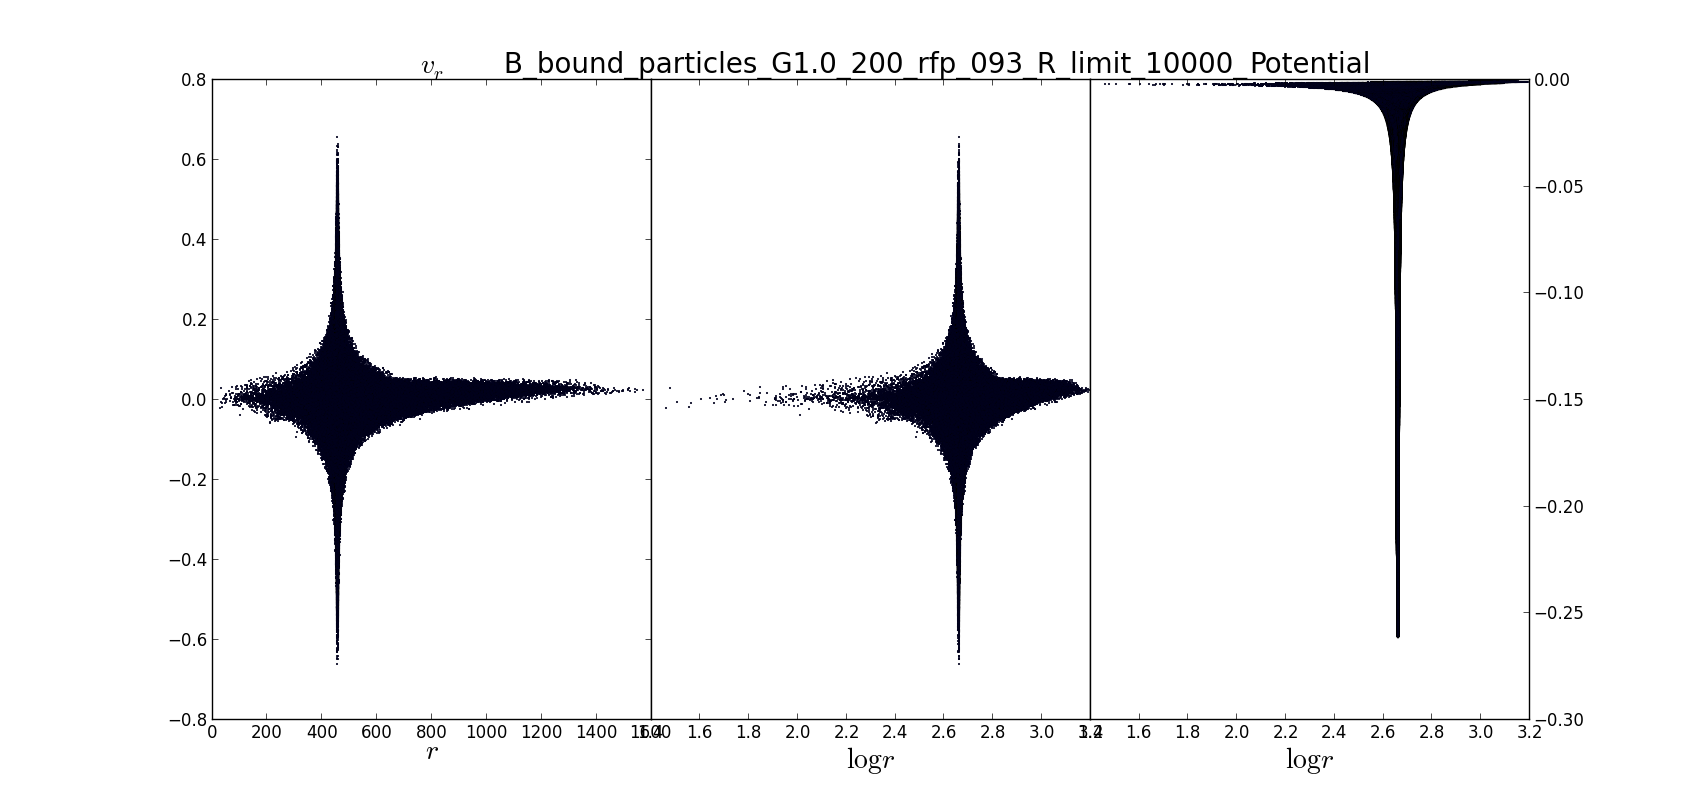
\includegraphics[width=1.0\linewidth]{img/B_rfp_vr_V_panel.png}
\caption{Final product of SIM B where all gravitationally unbound particles have been removed and the structures have had more time to equilibrate. Radial velocity vs. radius and logarithmic radius respectively. Gravitational potential vs. logarithmic radius. Notice how the outer regions now appear substantially different from the previous figure. There is a significant flattening of radial velocities in the scatterplots due to the removal of unbound particles as expected. The potential looks more or less the same apart from a slight contraction on the horizontal axis. This is natural as a removal of unbound particles that resided in the outer part of the structure lessens the gravitational pull outwards and the structure is therefore allowed to contract slightly more.}
\label{fig:test}
\end{figure}
\newpage

\begin{figure}
\centering
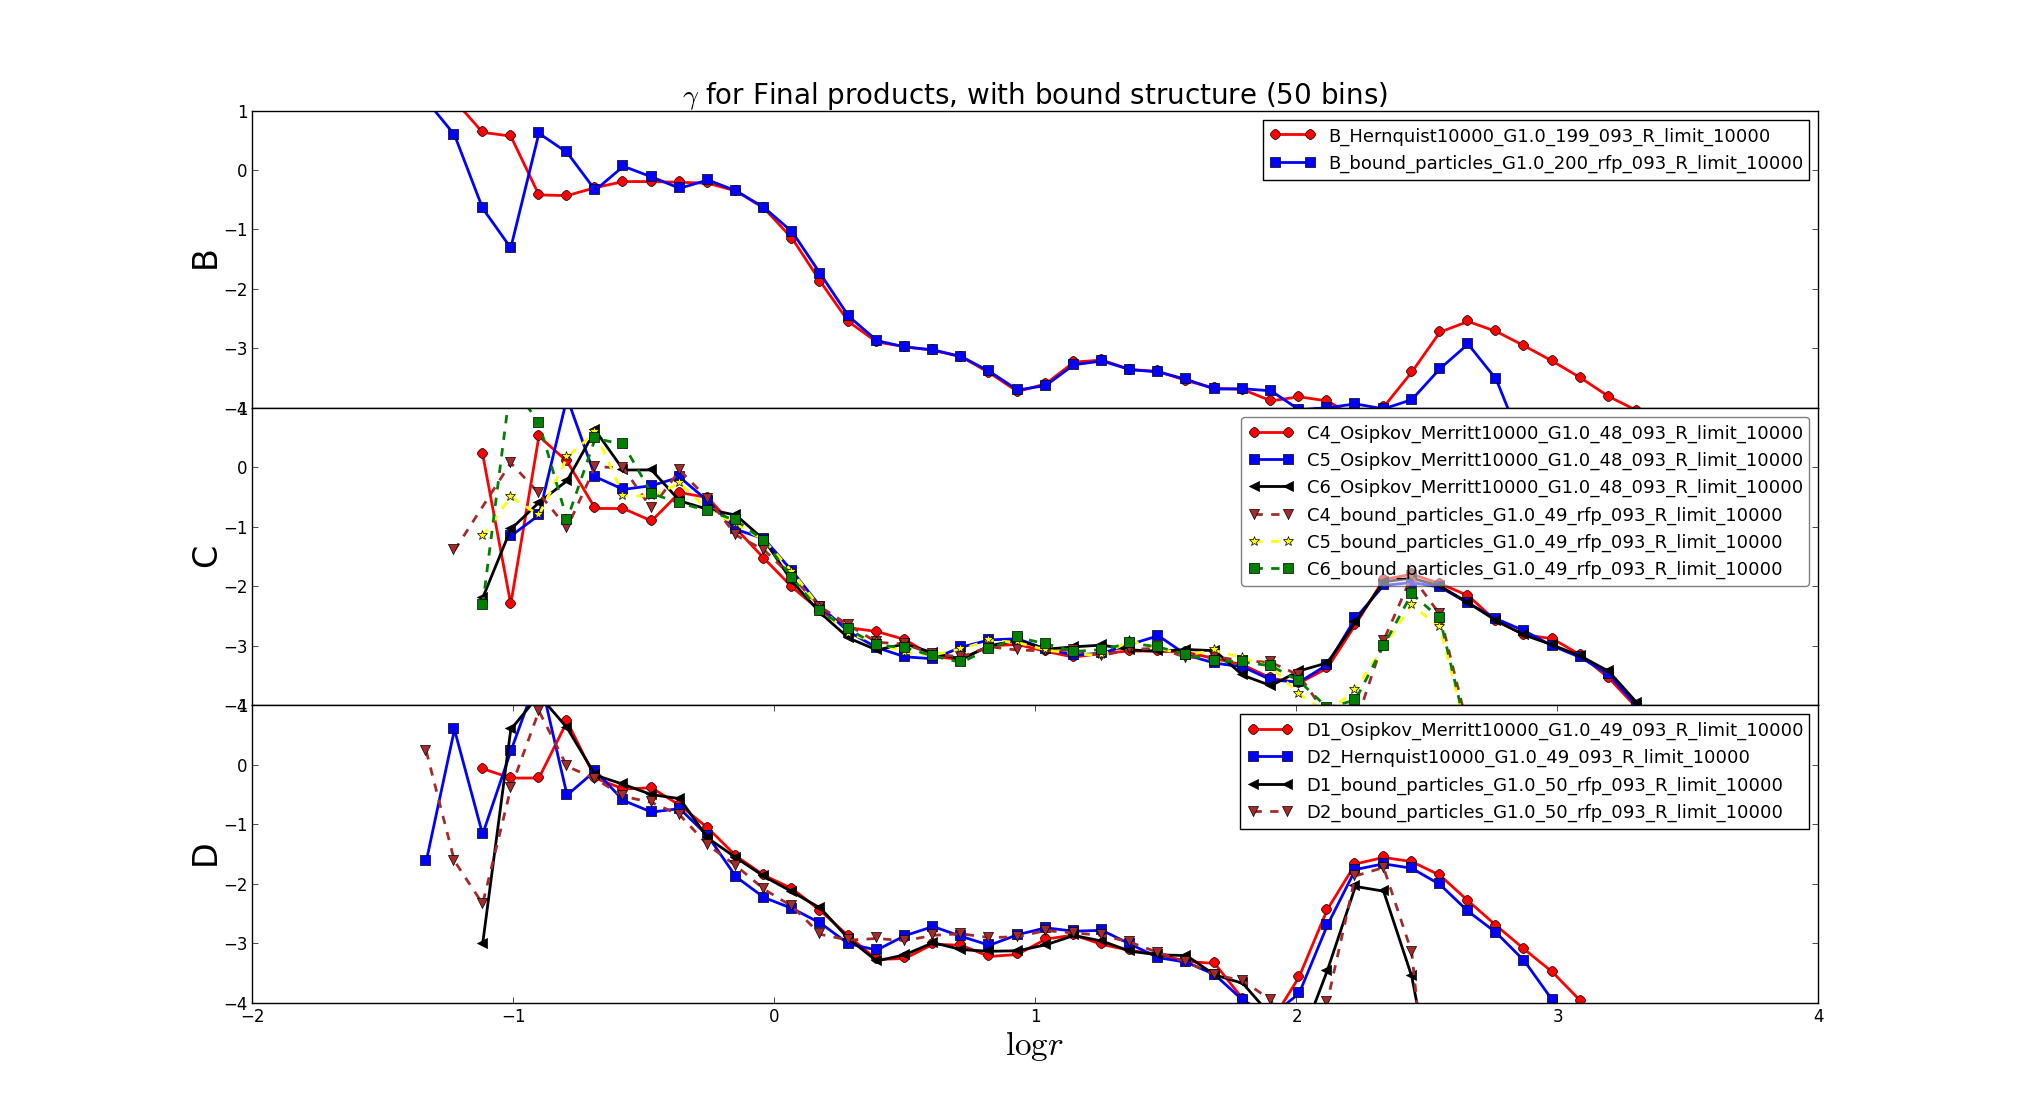
\includegraphics[width=1.0\linewidth]{img/BC4C5C6D1D2rfp_gamma_logr_panel.png}
\caption{The slope of the density profile, $\gamma$, vs. logarithmic radius for Final products of sims. B, $C_4$, $C_5$, $C_6$, $D_1$ and $D_2$ with structures containing all particles as well as same structures with only bound particles. 50 radial bins. $R_{limit} = 10^4$. Looking at the outer regions a clear effect is visible from the removal of gravitationally unbound particles: the final characteristic peak in the $\gamma$ profiles has dropped substantially.}
\label{fig:test}
\end{figure}

\begin{figure}
\centering
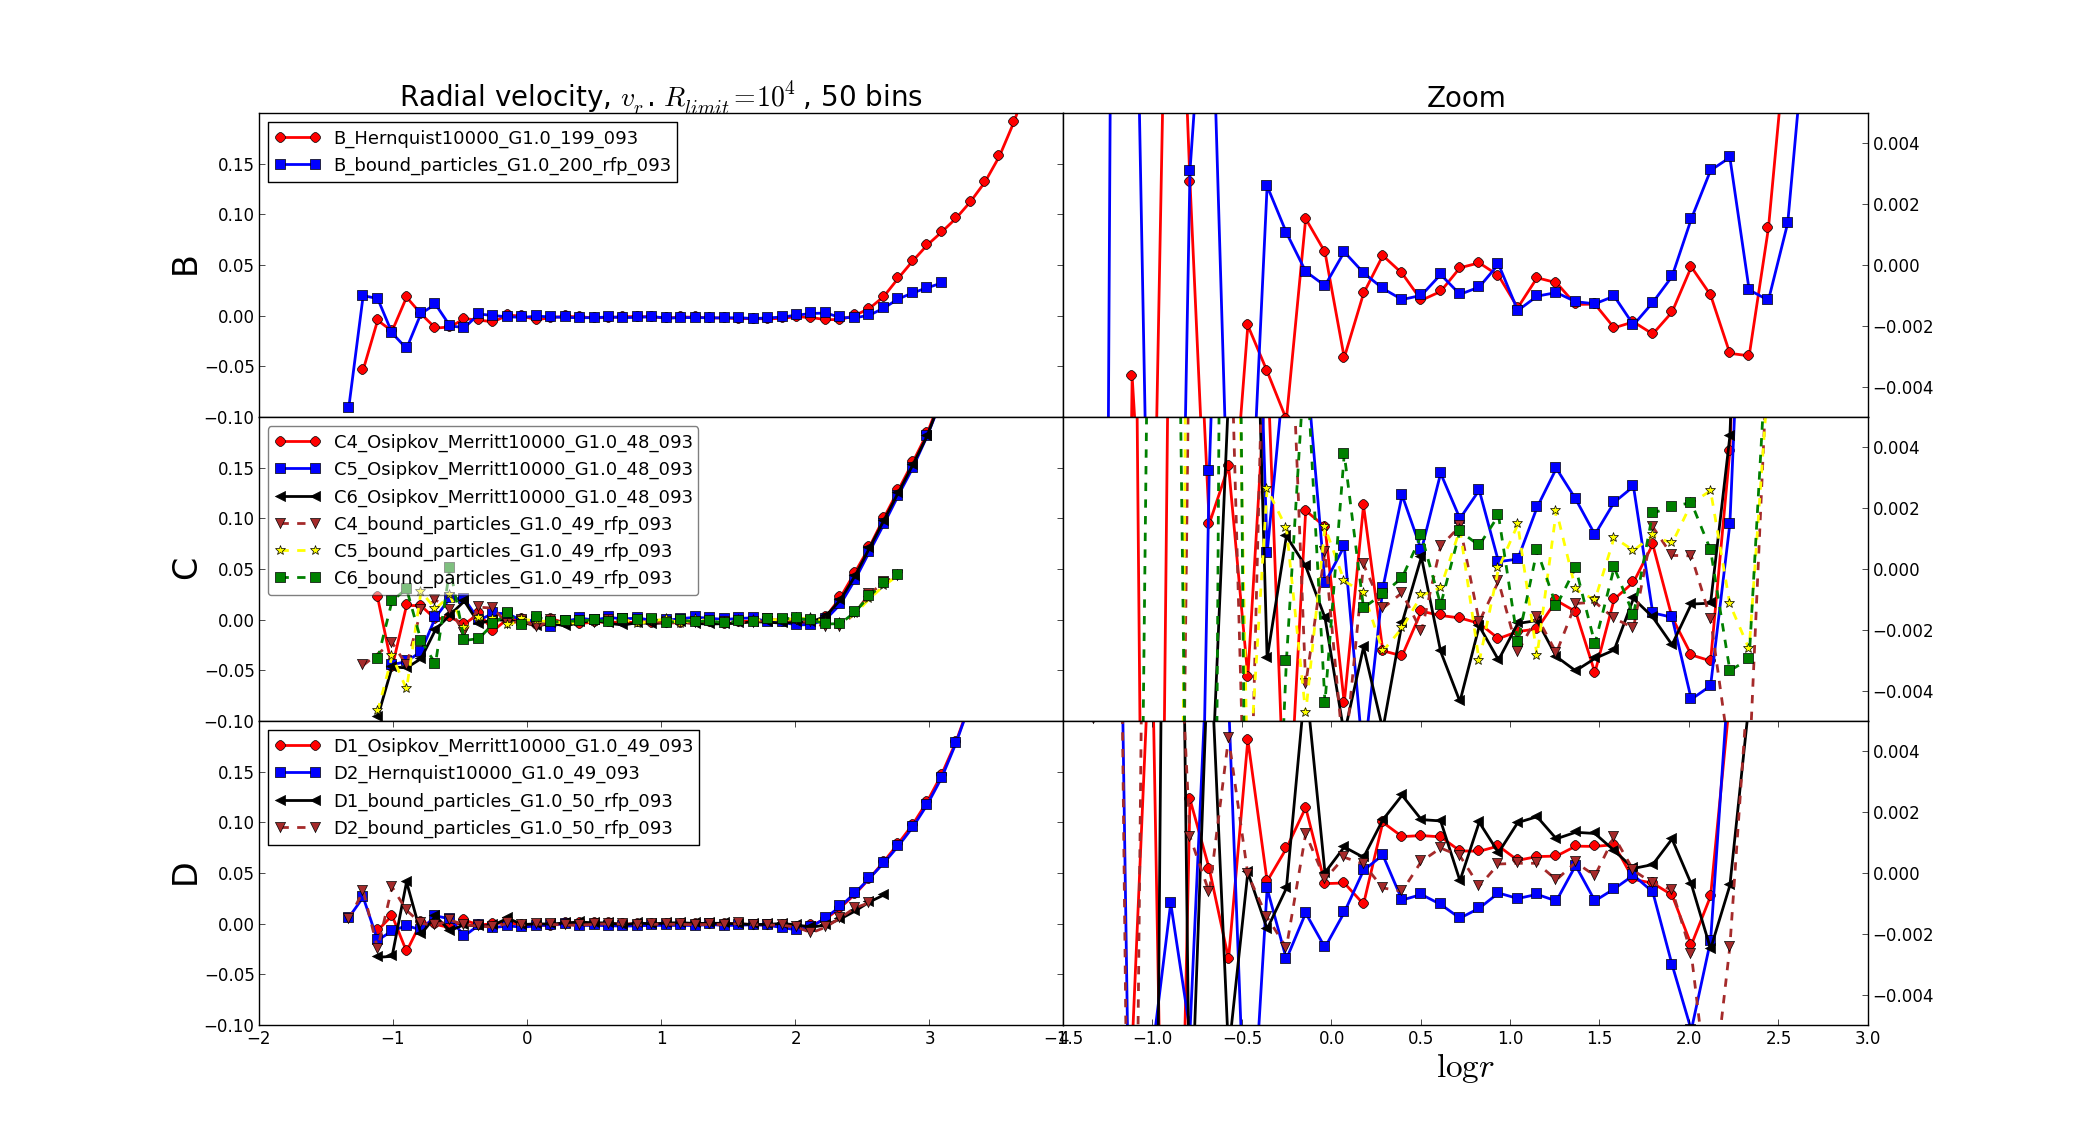
\includegraphics[width=1.0\linewidth]{img/BC4C5C6D1D2rfp_vr_logr.png}
\caption{Radial velocity vs. logarithmic radius for Final products of sims. B, $C_4$, $C_5$, $C_6$, $D_1$ and $D_2$ with structures containing all particles as well as same structures with only bound particles. 50 radial bins. $R_{limit} = 10^4$. The right panel shows zoom-ins of the left panel to investigate the mutual departures of the sims. around the middle region in more detail. Looking at the outer regions a clear effect is visible from the removal of gravitationally unbound particles: the increase in radial velocity has dropped substantially.
This might potentially make it possible to study the Jeans parameter attractor out to larger radii than previously.}
\label{fig:test}
\end{figure}